\chapter{Problem statement and formulation}\label{ch:problem-statement-and-formulation}

This chapter defines the painting placement problem, and its constraints.
First, let us define what a painting placement instance is.

\navesti{Painting placement isntance} is an ordered quadruple

\begin{equation}
    I = (P, F, L, \pi)\,,
    \label{eq:painting-placement-instance}
\end{equation}

where $P \subseteq (\nat^+, \nat^+)$ are painting dimensions (width$, $height pairs),
$F \subseteq \real^{|P|, |P|}$ is matrix defining flow between paintings,
$L \in \nat^+ \times \nat^+$ is layout dimension (width$\times$height pair)
and $\pi: \real \times \real \to \real$ is evaluation function.

An example of a painting placement instance is

\[
    I_1 = (\overbrace{((5,4),(8,5))}^{paintings},
    \overbrace{\begin{pmatrix}
                   0   & 5.8 \\
                   5.8 & 0
    \end{pmatrix}}^{flow},
    \overbrace{(15,7)}^{layout},
    \overbrace{f(x,y) = x+y)}^{evaluation function}\,.
\]

Instance $I_1$ has two paintings, the first one with dimensions $5\times4$, the second with $8\times5$.
The flow between them is $5.8$. The layout to which paintings are placed has a width $15$ and a height $7$.
The evaluation function is $f(x,y) = x+y$.

Next, each painting placement instance can have multiple solutions.

\navesti{Painting placement solution} is an ordered set of placement points
\begin{equation}
    S \subseteq (\natpos \times \natpos)^N  \,,
    \label{eq:painting-placement-solution}
\end{equation}
where $N$ is the size of the painting placement instance, i.e., the number of paintings.
For example, one solution $S_1$ for the instance $I_1$ can be

\[
    S_1 = ((0,0), (6,1)) \,.
\]

This means that the first painting's lower left corner will have coordinates $(0,0)$
and similarly $(6,1)$ for the second painting.
Illustration of both $I_1$ and $S_1$ can be seen in figure~\ref{fig:painting-placement-solution}.

\begin{figure}
    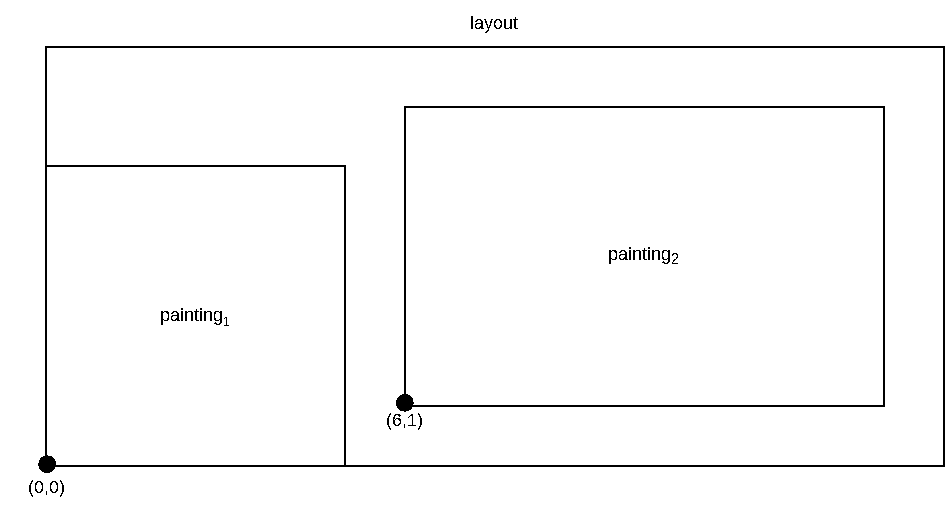
\includegraphics[width=0.9\textwidth, left]{painting_placement_solution}
    \caption[Example of a painting placement solution]{Example of a painting placement solution $S_1 = ((0,0), (6,1))$ for instance $I_1$.}
    \label{fig:painting-placement-solution}
\end{figure}

\newpage

Lastly, the painting placement solution needs to be evaluated.
Let's assume an instance $I$ and a set of all possible solutions $S$ to that instance.
Then, the painting placement problem is to find a minimum of a cost function $c: S \to \realpos$,
which can also be called an objective function, as


\begin{equation}
    \argmin_{x \in S} c(x) = \sum\limits_{i=1}^N\sum\limits_{j=i+1}^N f_{i,j}d(i, j) + \sum\limits_{i=1}^N \pi(i) + \lambda m(x) + \gamma n(x) \,,
    \label{eq:objective}
\end{equation}

where $f_{i,j}$ is flow between painting $i$ and $j$, $d(i,j)$ is their distance,
$\pi(i)$ is evaluation function applied to painting's $i$ lower left corner,
$m$ calculates number of overlapping paintings with penalization parameter $\lambda \in \real^+$
and $\gamma$ calculates the number of paintings placed outside of their allocated are
with penalization parameter $\gamma \in \real^+$.